\documentclass[a4paper]{article}
\usepackage[utf8]{inputenc}
\usepackage[russian,english]{babel}
\usepackage[T2A]{fontenc}
\usepackage[left=10mm, top=20mm, right=18mm, bottom=15mm, footskip=10mm]{geometry}
\usepackage{indentfirst}
\usepackage{amsmath,amssymb}
\usepackage[italicdiff]{physics}
\usepackage{graphicx}
\usepackage{caption}
\usepackage{float}
\usepackage{caption}
\renewcommand{\thefootnote}{\fnsymbol{footnote}}
\usepackage{tablefootnote}
\usepackage{footmisc}
\usepackage{textcomp}
\usepackage{multicol}
\usepackage[parfill]{parskip}
\usepackage{makecell}
\usepackage{array}  
\renewcommand\cellalign{cc} 
\renewcommand\cellgape{\Gape[2pt]} 
\usepackage[utf8]{inputenc}\newcommand{\approxtext}[1]{\ensuremath{\stackrel{\text{#1}}{\approx}}}
\usepackage[colorlinks=true, urlcolor=blue, linkcolor=blue, citecolor=blue]{hyperref}
\graphicspath{{images/}}
\DeclareGraphicsExtensions{.pdf,.png,.jpg}
\usepackage{wrapfig}
\captionsetup{labelformat=empty}
\usepackage{caption}
\captionsetup[figure]{name=Рисунок}
\captionsetup[table]{name=Таблица}
  
\title{\textbf{Отчет о выполненой лабораторной работе 2.3.1}}
\date{}
\author{Котляров Михаил, Б01-402}

\begin{document}

\maketitle
	
	\section{Введение}
	
	\textbf{Цель работы:}:  1)измерение объемов форвакуумной и высоковакуумной частей установки; 2) определение скорости откачки системы в стационарном режим, а также по ухудшению и по улучшению вакуума.\\

	\textbf{Оборудование:} вакуумная установка с манометрами: масляным, термопарным, и ионизационным; источник питания; видеокамера телефона.

\section{Экспериментальная установка}

    \begin{figure}[h]
        \center{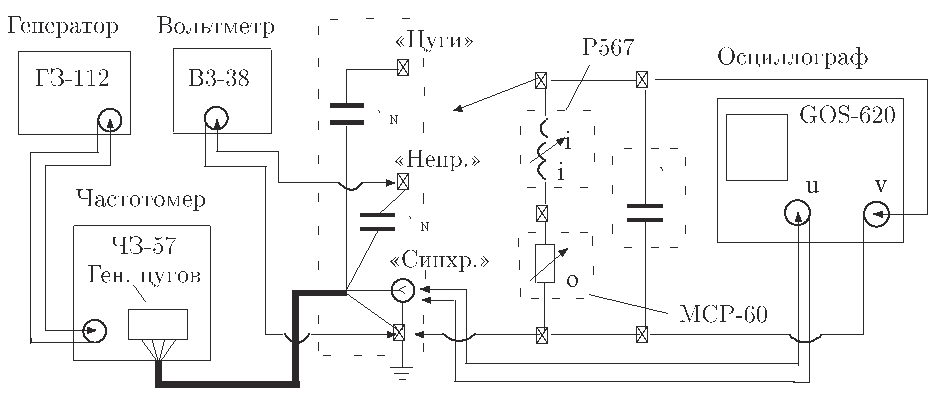
\includegraphics[width=0.8\textwidth]{Pictures/ustanovka}}
        \caption{Рис 1. Схема экспериментальной установки.}
        \label{ris:ustanovka}
    \end{figure}

    \paragraph{}
    Установка изготовлена из стекла и состоит из форвакуумного баллона (ФБ), высоковакуумного диффузионного насоса (ВН), высоковакуумного баллона (ВБ), масляного (М) и ионизационного (И) манометров, термопарных манометров ($M_1$ и $M_2$), форвакуумного насоса (ФН) и соединительных кранов (Рис. \ref{ris:ustanovka}).

    \paragraph{Маслянный манометр:}
    Представляет собой U-образную трубку, до половины наполненную вязким маслом, обладающим весьма низким давлением насыщенных паров. Так как плотность масла мала, $\rho = 0,885 г/см^3$ , то при помощи манометра можно измерить только небольшие разности давлений (до нескольких торр).

    \paragraph{Термопарный манометр:}
    Чувствительным элементом манометра является термопара, заключенная в стеклянный баллон. Устройство термопары пояснено на (Рис. \ref{ris:termoparni_monometr}). По нити накала НН пропускается ток постоянной величины. Термопара ТТ присоединяется к милливольтметру, показания которого определяются температурой нити накала и зависят от отдачи тепла в окружающее пространство. Потери тепла определяются теплопроводностью нити и термопары, теплопроводностью газа, переносом тепла конвективными потоками газа внутри лампы и теплоизлучением нити (инфракрасное тепловое излучение). В обычном режиме лампы основную роль играет теплопроводность газа. При давлениях >1 торр теплопроводность газа, а вместе с ней и ЭДС термопары практически не зависят от давления газа, и прибор не работает. При улучшении вакуума средний свободный пробег молекул становится сравнимым с диаметром нити, теплоотвод падает и температура спая возрастает. При вакууме $\sim 10^{-3}$ торр теплоотвод, осуществляемый газом, становится сравнимым с другими видами потерь тепла и температура нити становится практически постоянной. Градуировочная кривая термопарного манометра приведена на (Рис. \ref{ris:termopara_graduirovka}).

    \begin{figure}[h]
    \centering
    \begin{minipage}{0.3\textwidth}
        \centering
        \includegraphics[width=0.7\textwidth]{Pictures/termoparni_monometr}
        \caption{Рис 2. Схема термопарного манометра.}
        \label{ris:termoparni_monometr}
    \end{minipage}\hfill
    \begin{minipage}{0.7\textwidth}
        \centering
        \includegraphics[width=0.7\textwidth]{Pictures/termopara_graduirovka}
        \caption{Рис3. Градуировочная кривая термопарного манометра.}
        \label{ris:termopara_graduirovka}
    \end{minipage}
    \end{figure}

    \paragraph{Ионизационный манометр:}
    Схема ионизационного манометра изображена на (Рис. \ref{ris:ionizacionni_monometr}). Он представляет собой трехэлектродную лампу. Электроны испускаются накаленным катодом и увлекаются электрическим полем к аноду, имеющему вид спирали. Проскакивая за ее витки,электроны замедляются полем коллектора и возвращаются к катоду, а от него вновь увлекаются к аноду. Прежде чем осесть на аноде, они успевают много раз пересечь пространство между катодом и коллектором. На своем пути электроны ионизуют молекулы газа. Ионы, образовавшиеся между анодом и коллектором, притягиваются полем коллектора и определяют его ток. Ионный ток в цепи коллектора пропорционален плотности газа и поэтому может служить мерой давления. Калибровка манометра верна, если остаточным газом является воздух. Накаленный катод ионизационного манометра перегорает, если давление в системе превышает $10^{-3}$ торр. Поэтому включать ионизационный манометр можно, только убедившись по термопарному манометру, что давление в системе не превышает $10^{-3}$ торр. При измерении нить ионизационного манометра сильно греется. При этом она сама, окружающие ее электроды и стенки стеклянного баллона могут десорбировать поглощенные ранее газы. Выделяющиеся газы изменяют давление в лампе и приводят к неверным показаниям. Поэтому перед измерениями ионизационный манометр прогревается (обезгаживается) в течение 10–15 мин. Для прогрева пропускается ток через спиральный анод лампы.

    \vspace{1cm}

    \begin{figure}[h]
        \center{\includegraphics[width=0.3\textwidth]{Pictures/ionizacionni_monometr}}
        \caption{Рис 4. Схема ионизационного манометра.}
        \label{ris:ionizacionni_monometr}
    \end{figure}

    \newpage

    \paragraph{Диффузионный насос:}
    Откачивающее действие диффузионного насоса основано на диффузии (внедрении) молекул разреженного воздуха в струю паров масла. Попавшие в струю молекулы газа увлекаются ею и уже не возвращаются назад. Устройство одной ступени масляного диффузионного насоса схематически показано на (Рис. \ref{ris:diffuzionni_nasos}) (в лабораторной установке используется несколько откачивающих ступеней). Масло, налитое в сосуд А, подогревается электрической печкой. Пары масла поднимаются по трубе Б и вырываются из сопла В. Струя паров увлекает молекулы газа,которые поступают из откачиваемого сосуда через трубку ВВ. Дальше смесь попадает в вертикальную трубу Г. Здесь масло осаждается на стенках трубы и маслосборников и стекает вниз, а оставшийся газ через трубу ФВ откачивается форвакуумным насосом. Диффузионный насос работает наиболее эффективно при давлении, когда длина свободного пробега молекул воздуха примерно равна ширине кольцевого зазора между соплом В и стенками трубы ВВ. В этом случае пары масла увлекают молекулы воздуха из всего сечения зазора. Давление насыщенных паров масла при рабочей температуре, создаваемой обогревателем сосуда А, много больше $5\cdot10^{-2}$ торр. Именно поэтому пары масла создают плотную струю, которая и увлекает с собой молекулы газа. Если диффузионный насос включить при давлении, сравнимом с давлением насыщенного пара масла, то последнее никакой струи не создаст и масло будет просто окисляться и угорать.

    \begin{figure}[h]
    \centering
        \includegraphics[width=0.6\textwidth]{Pictures/diffuzionni_nasos}
        \caption{Рис 5. Схема одной ступени диффузионного насоса.}
        \label{ris:diffuzionni_nasos}
    \end{figure}
	
	\section{Процесс откачки}
Производительность насоса определяется скоростью откачки $W$ (л/с): $W$ - это объем газа, удаляемого из сосуда при данном давлении за единицу времени. Скорость откачки форвакуумного насоса равна ёмкости воздухозаборной камеры, умноженной на число оборотов в секунду.\\
Обозначим через $Q_\text{д}$ количество газа, десорбирующегося с поверхности откачиваемого объема в единицу времени, через $Q_\text{и}$ - количество газа, проникающего в единицу времени в этот объем извне - через течи, через $Q_\text{н}$ - поток газа, поступающего из насоса назад в откачивающую систему. Будем измерять их в единицах $PV$. Основное уравнение, описывающее процесс откачки, имеет вид
\begin{equation*}
	-VdP = (PW - Q_\text{д} - Q_\text{и} - Q_\text{н})dt.
	\eqno(1)
\end{equation*}
При достижении предельного вакуума (давление $P_\text{пр}$)
\begin{equation*}
	\frac{dP}{dt} = 0,
\end{equation*}
так что
\begin{equation*}
	PW = Q_\text{д} + Q_\text{и} + Q_\text{н}.
	\eqno(2)
\end{equation*}
Из этого уравнения получаем
\begin{equation*}
	W = \frac{\displaystyle \sum Q_i}{P_\text{пр}}.
\end{equation*}
Обычно $Q_\text{и}$ постоянно, а $Q_\text{д}$ и $Q_\text{н}$ слабо зависят от времени. Считая скорость откачки $W$ постоянной, уравнение (1) можно проинтегрировать и, используя (2), получить
\begin{equation*}
	P - P_\text{пр} = (P_0 - P_\text{пр}) e^{-\frac{t}{\tau}},
	\eqno(3)
\end{equation*}
где $\tau = \frac{V}{W}$ является мерой эффективности откачки системы.\\
Для количества газа, протекающего через трубу в условиях высокого вакуума справедлива формула
\begin{equation*}
	\frac{d(PV)}{dt} = \frac{4}{3} r^3 \sqrt{\frac{2\pi RT}{\mu}}\frac{P_2 - P_1}{L}.
	\eqno(4)
\end{equation*}
Пренебрежем давлением $P_1$ у конца обращенного к насосу. Будем измерять количество газа, покидающего установку при давлении $P = P_2$. Пропускная способность трубы
\begin{equation*}
	C_\text{тр} = \left(\frac{dV}{dt}\right) = \frac{4}{3} \frac{r^3}{L} \sqrt{\frac{2\pi RT}{\mu}}.
	\eqno(5)
\end{equation*}
Для пропускной способности отверстия имеем формулу 
\begin{equation*}
	C_\text{отв} = S\frac{\bar{v}}{4}.
	\eqno(6)
\end{equation*}

\section{Приборы и данные}
\begin{itemize}
    \item Вакуумметр Мерадат-ВИТ19ИТ2, тип первичного преобразователя ПМИ-2, погрешность в диапазоне $1\cdot10^{-4}$ Па до $5\cdot10^{-2}$ Па 35\% от измеряемой величины.
	\item Вакуумметр Мерадат-ВИТ16Т4, тип первичного преобразователя ПМТ-2, погрешность в диапазоне $1\cdot10^{-3}$ торр до $0,2$ торр 30\% от измеряемой величины.
	\item Масляной манометр (плотность масла $\rho = 0,885 \ \frac{\text{г}}{\text{см}^3}$), погрешность измеряющей линейки 1 мм.
	\item Источник питания GPR-711H30D, погрешность измерения $\pm(0,5 \% +2 ед.)$.
	\item Термогигрометр с функцией отображения давления testo 622, погрешность измерения давления 3 гПа, температуры - 0,4 $^\circ C$, влажности - 2\% в диапазоне от 0 до 90 \%.
\end{itemize}

\section{Выполнение}


Начальные параметры окружающей среды
\begin{equation*}
	t = 22,2 ^\circ C,
\end{equation*}
\begin{equation*}
	P_0 = 99,00 \text{ кПа},
\end{equation*}
\begin{equation*}
	\varphi = 41,6 \%.
\end{equation*}

\subsection{Измерение объема баллонов}
\begin{enumerate}
\item Ход выполнения
Перед началом работы убедимся, что кран $K_2$ закрыт, а остальные открыты. Откроем кран $K_2$ на 1-2 минуты, чтобы воздух заполнил всю установку. Закроем краны $K_5$ и $K_6$. В этих кранах запирается $V_{56} = 50 \text{ см}^3$ воздуха при атмосферном давлении. Закроем кран $K_2$ и включим форвакуумный насос. В течение двух минут насос будет откачивать сам себя. Затем откроем кран $K_2$ и начнем откачку установки. После откачки закроем кран $K_2$, тем самым отсоединив установку от форвакуумного насоса. Давление на манометре ВИТ16 $P_\text{вак} = 1,8 \cdot 10^{-2}$ торр. Закроем кран $K_3$, отсоединив высоковакуумную часть от форвакуумной. Закроем кран $K_4$ для подготовки масляного манометра к измерениям. Откроем кран $K_5$, распространив запертый в капилляре 5-6 атмосферный воздух по всей форвакуумной части. Установившееся давление зафиксируем на манометре.
\begin{align*}
    h_1 &= 11,6 \pm 0,1\text{ см}, & 
    h_2 &= 37,9 \pm 0,1\text{ см}, & 
    \Delta h' &= 26,3 \pm 0,2\text{ см}.
\end{align*}
Откроем кран $K_3$, заполнив высоковакуумную часть воздухом. Зафиксируем давление на масляном манометре.
\begin{align*}
	h_3 &= 16,4 \pm 0,1\text{ см}, & 
	h_4 &= 33,3 \pm 0,1\text{ см}, & 
	\Delta h'' &= 16,9 \pm 0,2\text{ см}.
\end{align*}
Закроем кран $K_4$. Теперь рассчитаем объем  форвакуумной $V_\text{фв}$ и высоковакуумной $V_\text{вв}$ частей с помощью закона Бойля-Мариотта
\begin{equation*}
	P_1V_1= P_2V_2.
\end{equation*}
\begin{equation*}
	P_0V_{56} = (V_{56} + V_\text{фв})\rho_{\text{масло}} g \Delta h',
\end{equation*}
\begin{equation*}
	V_\text{фв} = V_{56}(\frac{P_0}{\rho_{\text{масло}} g \Delta h'} - 1) = 0,05 \cdot (\frac{99000}{885 \cdot 9,81 \cdot 0,263} - 1) \approx 2,118 \text{ л},
\end{equation*}
\begin{equation*}
	V_\text{вв} = V_{56}(\frac{P_0}{\rho_{\text{масло}} g \Delta h''} - 1) - V_\text{фв} = 0,05 \cdot (\frac{99000}{885 \cdot 9,81 \cdot 0,169} - 1) - 2,118 \approx  1,206 \text{ л},
\end{equation*}
\begin{equation*}
\sigma_{V_\text{фв}} = (V_\text{фв} + V_{56}) \cdot \sqrt{\left( \frac{V_\text{фв}}{V_\text{фв} + V_{56}} \frac{\sigma_{V_{56}}}{V_{56}} \right)^2 + \left(\frac{\sigma_\rho}{\rho}\right)^2 + \left(\frac{\sigma_h}{h}\right)^2 + \left(\frac{\sigma_P}{P}\right)^2} =
\end{equation*}
\begin{equation*}
= \sqrt{\left( 0,004 \right)^2 + \left(0,002\right)^2 + \left(0,017\right)^2 + \left(0,007\right)^2} = 0,018 \text{ л},
\end{equation*}
\begin{equation*}
\sigma_{V_\text{вв}}  = 0,060 \text{ л},
\end{equation*}

\item Итого значения для объемов $V_\text{фв} = 2,118 \pm 0,018$ ($\varepsilon_\text{фв} =0,87 \%$), $V_\text{вв} = 1,206 \pm 0,060$ ($\varepsilon_\text{вв} =5,00 \%$).

\subsection{Получение высокого вакуума и измерение скорости откачки}

\item Откроем все краны и откачаем всю систему до давления $\sim 1\cdot 10^{-2}$ торр. После этого приступим к откачке высоковакуумного баллона с помощью диффузионного насоса. Выставим на источнике питания ток $I = 0,6$ А, подождем приблизительно 5 минут, чтобы масло прогрелось, а затем постепенно установим ток 1,27 А. Дождемся давления  $\sim 3\cdot 10^{-4}$ торр и запустим ионизационный манометр. После того, как давление достигнет $\sim 1\cdot 10^{-4}$ торр, проведем дегазацию.\\
	Выждав установленное время дегазации, давление достигло $P_{\text{пр}} = (8,30 \pm 2,91)  \cdot 10^{-5}$ торр. Теперь будем фиксировать изменение давления от времени с помощью видеокамеры телефона. Для этого закроем кран $K_3$, отключив тем самым откачку высоковамуумного баллона. Будем фиксировать ухудшение вакуума до давления $\sim 5\cdot 10^{-4}$, а затем опять откроем кран $K_3$ и будем фиксировать улучшение. Проделаем этот опыт два раза.\\
	По полученным данным построим зависимость $P(t)$. Также для экспоненциального участка при улучшении давления построим график зависимости $\ln(P - P_{\text{пр}})$.
\begin{figure}[h!]
\centering{\includegraphics[width=1\textwidth]{Graphics/series2_extended.png}}
\caption[]{\label{} График 1. График зависимости давления от времени $P(t)$ для первой серии}
\end{figure}
\begin{figure}[h!]
\centering{\includegraphics[width=1\textwidth]{Graphics/series1_extended.png}}
\caption[]{\label{} График 2. График зависимости давления от времени $P(t)$ для второй серии}
\end{figure}
\clearpage
\begin{figure}[h!]
\centering{\includegraphics[width=1\textwidth]{Graphics/lnP_2.png}}
\caption[]{\label{} График 3. График зависимости логарифма разности давления и предельного давления от времени $\ln(P - P_{\text{пр}})$ для первой серии}
\end{figure}
\begin{figure}[h!]
\centering{\includegraphics[width=1\textwidth]{Graphics/lnP_1.png}}
\caption[]{\label{} График 4. График зависимости логарифма разности давления и предельного давления от времени $\ln(P - P_{\text{пр}})$ для второй серии}
\end{figure}
\clearpage
Получившиеся параметры прямых
\begin{equation*}
    k_1^{lin} = (1.324 \pm 0,006) \cdot 10^{-5} \ \frac{\text{торр}}{\text{с}}, 
\end{equation*}
\begin{equation*}
    k_2^{lin} = (1.314 \pm 0,005) \cdot 10^{-5} \ \frac{\text{торр}}{\text{с}}, 
\end{equation*}
\begin{equation*}
    \frac{1}{k_1^{exp}} = \tau_1 = (5,01 \pm 0,07) \ \text{с}, 
\end{equation*}
\begin{equation*}
    \frac{1}{k_2^{exp}} = \tau_2 = (5,35 \pm 0,05) \ \text{с},
\end{equation*}
\begin{equation*}
    \tau = \bar{\tau} = \frac{\tau_1 + \tau_2}{2} = (5,18 \pm 0,06) \ \text{с}.
\end{equation*}

\item Рассчитаем скорость откачки $W$
\begin{equation*}
    W = \frac{V_\text{вв}}{\tau} = \frac{1,206}{5,18} = 0,233 \ \frac{\text{л}}{\text{с}},
\end{equation*}
\begin{equation*}
    \sigma_W =  W \sqrt{\left(\frac{\sigma_{V_\text{вв}}}{V_\text{вв}}\right)^2 +\left(\frac{\sigma_{\tau}}{\tau}\right)^2} = 0,233 \cdot \sqrt{\left( 0,05\right)^2 + \left(0,01\right)^2} = 0,012 \ \frac{\text{л}}{\text{с}},
\end{equation*}
\begin{equation*}
    \varepsilon_W =  5,14 \%.
\end{equation*}

\item Оценим величину потока газа $Q_{\text{н}}$, поступающего из насоса назад в откачиваемую систему. Воспользуемся уравнением
\begin{equation*}
      V_{\text{вв}}dP = (Q_\text{д} + Q_\text{и})dt.
\end{equation*}
В качестве $k = \frac{dP}{dt}$ возьмем $\bar{k}= \frac{k_1^{lin} + k_2^{lin}}{2} = (1,319 \pm 0,006) \cdot 10^{-5} \ \frac{\text{торр}}{\text{с}}$. Зная также, что $PW = Q_\text{д} + Q_\text{и} + Q_\text{н}$, получим
\begin{equation*}
      Q_\text{н} = P_{\text{пр}} W - k V_{\text{вв}} = 8,30 \cdot 10^{-5} \cdot 0,233 - 1,319 \cdot 10^{-5} \cdot 1,206 = 3,5 \cdot 10^{-6} \frac{\text{торр} \cdot \text{л}}{\text{с}}.
\end{equation*}
Посчитаем погрешность
\begin{equation*}
      \sigma_{Q_\text{н}} = \sqrt{\left(\sigma_{P_{\text{пр}}} W\right)^2 + \left({P_{\text{пр}}} \sigma_W\right)^2} + \sqrt{\left(\sigma_{V_{\text{вв}}} k\right)^2 + \left({V_{\text{вв}}} \sigma_k\right)^2} =
\end{equation*}
\begin{equation*}
= 10^{-3} \cdot \sqrt{\left(6,762\right)^2 + \left(0,992\right)^2} + \sqrt{\left(0,793\right)^2 + \left(0,067\right)^2} = 7,6 \cdot 10^{-6} \frac{\text{торр} \cdot \text{л}}{\text{с}}.
\end{equation*}
Исходя из этого можно сделать вывод, что таким методом можно оценить только приблизительный порядок величины.

\subsection{Метод введения искуственной течи}
\item Откроем кран $K_5$ и введем в сестему искуственную течь. Через 3-5 минут измерим установившееся давление. $P_{\text{уст}} = (1,60 \pm 0,56) \cdot 10^{-4}$. Также зафиксируем давление со стороны форвакуумной части.\\ $P_{\text{фв}} = (5,40 \pm 1,62) \cdot 10^{-3}$. С помощью соотношений $P_{\text{пр}} W = Q_1$, $P_{\text{уст}} W = Q_1 + \frac{d(PV)_{\text{кап}}}{dt}$ а также формулы (4), исключив$WQ_1$ найдем скорость откачки системы $W$. Размеры капилляра $r = 0,8 \pm 0,1 \ \text{мм}$, $L = 10,8 \pm 0,1 \ \text{см}$.
\begin{equation*}
      C_\text{кап} = \frac{4}{3} \frac{(0,8\cdot 10^{-3})^3}{10,8 \cdot 10^{-2}} \sqrt{\frac{2 \cdot 3,1415 \cdot 8,31 \cdot (273 + 22,2)}{29 \cdot 10^{-3}}} = 5,76 \cdot 10^{-7} \ \frac{\text{м}^3}{\text{с}},
\end{equation*}
\begin{equation*}
      \sigma_{C_\text{кап}} = C_\text{кап} \sqrt{\left(\frac{3\sigma_r}{r}\right)^2 + \left(\frac{\sigma_L}{L}\right)^2 + \left(\frac{\sigma_T}{T}\right)^2} =
\end{equation*}
\begin{equation*}
= 5,76 \cdot 10^{-7} \cdot \sqrt{\left(0,375\right)^2 + \left(0,009\right)^2 + \left(0,001\right)^2} = 2,16 \cdot 10^{-7} \ \frac{\text{м}^3}{\text{с}},
\end{equation*}
\begin{equation*}
      W = \frac{C_\text{кап}(P_{\text{фв}} - P_{\text{уст}})}{P_{\text{уст}} - P_{\text{пр}}} = \frac{2,16 \cdot 10^{-7} \cdot (5,4 \cdot 10^{-3} - 1,6 \cdot 10^{-4} )}{1,6 \cdot 10^{-4} - 8,3 \cdot 10^{-5}} = 3,92 \cdot 10^{-5} \ \frac{\text{м}^3}{\text{с}} = 0,04 \ \frac{\text{л}}{\text{с}},
\end{equation*}
\begin{equation*}
      \sigma_W = C_\text{кап} \sqrt{\left(\frac{\partial W}{\partial P_{\text{фв}}}\frac{\sigma{P_{\text{фв}}}}{C_\text{кап}}\right)^2 + \left(\frac{\partial W}{\partial P_{\text{уст}}}\frac{\sigma{P_{\text{уст}}}}{C_\text{кап}}\right)^2 + \left(\frac{\partial W}{\partial P_{\text{пр}}}\frac{\sigma{P_{\text{пр}}}}{C_\text{кап}}\right)^2 + \left(\frac{\partial W}{\partial C_\text{кап}}\frac{\sigma{C_\text{кап}}}{C_\text{кап}}\right)^2} =
\end{equation*}
\begin{equation*}
= 5,76 \cdot 10^{-7} \cdot \sqrt{\left(2\right)^2 + \left(5\right)^2 + \left(3\right)^2 + \left(3\right)^2} = 3,77 \cdot 10^{-5} \ \frac{\text{м}^3}{\text{с}},
\end{equation*}
\begin{equation*}
      \varepsilon_W = 96 \%.
\end{equation*}

Таким образом величина $W \approx  0,04 \ \frac{\text{л}}{\text{с}}$ получена с огромной погрешностью, что говорит о неточности такого метода измерения.

\end{enumerate}

\section{Результаты и обсуждения}
\begin{enumerate}
\item Вычисленные объёмы форвакуумного и высоковакуумного баллонов получены с хорошей точностью. \\$V_\text{фв} = 2,118 \pm 0,018$ ($\varepsilon_\text{фв} =0,87 \%$), $V_\text{вв} = 1,206 \pm 0,060$ ($\varepsilon_\text{вв} =5,00 \%$).
\item По графикам 1-4 отчетливо видно, что давление растет линейно со временем при просачивании воздуха, а откачка идет по экспоненте.\\ С помощью графиков 3-4 получили характерное время откачки $\tau = (5,18 \pm 0,06) \ \text{с}$.
\item С помощью двух методов мы определили скорость откачки $W$: по улучшению вакуума (метод 1) и по введению искусственной течи (метод 2).
\begin{table}[h!]
    \centering
    \begin{tabular}{|c|c|c|c|}
        \hline
        Метод & $W,\ \frac{\text{л}}{\text{с}}$ & $\sigma_W,\ \frac{\text{л}}{\text{с}}$ & $\varepsilon_W,\ \%$ \\
        \hline
        1 & $0{,}233$ & $0{,}012$ & $5{,}1$ \\ \hline
        2 & $0{,}039$ & $0{,}038$ & $96{,}1$ \\
        \hline
    \end{tabular}
    \caption{Сравнение результатов измерения скорости откачки разными методами}
\end{table}
\\Первый метод оказался довольно точным, погрешность составила всего 5 \%. Второй метод не подходит для измерений с большой точностью, а только для грубой оценки. Погрешность радиуса дает больший клад, т.к. зависимость от куба, поэтому погрешность почти равна самой величине.
\item Оцененное значение для потока газа $Q_\text{н} =  (3,5 \pm 7,6) \cdot 10^{-6} \frac{\text{торр} \cdot \text{л}}{\text{с}}$ также получено исключительно оценочно, о этом можно судить исходя из погрешности. 
\end{enumerate}

\section{Выводы}
Были вычислены с помощью вакуумной установки, манометров и закона Бойля-Мариотта объемы форвакуумного и высоковакуумного баллонов. С помощью двух методов определили скорость откачки насоса. Построили графики зависимостей $P(t)$ и $\ln(P - P_\text{пр})$. Оценили значение для потока газа, поступающего из насоса назад в откачиваемую систему.

\end{document}